\section{Methodology}
\label{sec:methodology}

This section presents the \dreamprice{} architecture, training procedure, and causal identification strategy. The approach combines a recurrent state-space model with a \mamba{} selective state-space backbone \citep{dao2024mamba2}, DRAMA-style decoupled posteriors \citep{rajbhandari2024drama}, a causally-constrained demand decoder, and MOPO-style offline pessimism \citep{yu2020mopo}. The training recipe follows \dreamer{} \citep{hafner2023dreamerv3} with adaptations for retail pricing and offline learning.

\subsection{Problem Formulation}

Retail pricing is formulated as a partially observable Markov decision process (POMDP) in which the decision-maker observes prices, quantities sold, promotions, and store demographics, but the underlying state governing demand dynamics is only partially observable. The true state $s_t$ comprises demand state (consumer preferences, inventory effects, substitution structure), competitor state (rival prices and promotions, which are unobserved in the Dominick's dataset), and seasonal state (calendar effects, holidays, macroeconomic conditions). The observation $x_t$ at time $t$ includes per-SKU prices, units sold, promotion indicators, lagged demand and price features, rolling statistics, and store demographics. The action $a_t$ is a vector of price multipliers over $K$ SKUs, discretized to 21 levels per SKU: $a_t \in \{0.90, 0.91, \ldots, 1.10\}^K$, representing percentage adjustments relative to a baseline price. The reward combines gross margin with a volatility penalty and a margin floor penalty to discourage degenerate strategies such as perpetual deep discounts or excessive price churn. The transition dynamics are unknown and must be learned from data.

\begin{definition}[Retail Pricing POMDP]
\label{def:pomdp}
A retail pricing POMDP is a tuple $(\mathcal{S}, \mathcal{X}, \mathcal{A}, \mathcal{T}, \mathcal{O}, \mathcal{R}, \gamma)$ where:
\begin{itemize}[leftmargin=*]
\item $\mathcal{S}$ is the latent state space comprising demand, competitor, and seasonal components.
\item $\mathcal{X}$ is the observation space: per-SKU prices, units sold, promotions, demographics, and derived features.
\item $\mathcal{A} = \{0.90, 0.91, \ldots, 1.10\}^K$ is the action space of discrete price multipliers.
\item $\mathcal{T}(s_{t+1} \mid s_t, a_t)$ is the unknown transition kernel.
\item $\mathcal{O}(x_t \mid s_t)$ is the observation model.
\item $\mathcal{R}(s_t, a_t)$ is the reward: gross margin minus volatility penalty minus margin floor penalty.
\item $\gamma \in (0, 1)$ is the discount factor.
\end{itemize}
\end{definition}

The objective is to learn a world model that approximates $\mathcal{T}$ and $\mathcal{O}$ from offline historical data, then use imagination-based policy optimization to find a pricing policy that maximizes expected cumulative discounted reward \citep{sutton2018reinforcement, hafner2023dreamerv3}.

\begin{figure}[t]
\centering
\resizebox{0.92\textwidth}{!}{%
\begin{tikzpicture}[
  node distance=0.7cm and 1.2cm,
  box/.style={draw, rounded corners=3pt, minimum width=2.4cm, minimum height=0.7cm, align=center, font=\small},
  inputbox/.style={box, fill=blue!8, draw=blue!60!black},
  encoderbox/.style={box, fill=green!10, draw=green!50!black},
  backbonebox/.style={box, fill=violet!12, draw=violet!60!black, minimum width=3.0cm, minimum height=0.9cm},
  decoderbox/.style={box, fill=red!8, draw=red!50!black},
  rewardbox/.style={box, fill=orange!10, draw=orange!60!black},
  headbox/.style={box, fill=teal!10, draw=teal!60!black},
  priorbox/.style={box, fill=blue!8, draw=blue!60!black},
  arr/.style={-{Stealth[length=2.5mm]}, thick},
  garr/.style={-{Stealth[length=2.5mm]}, thick, gray!70},
  lbl/.style={font=\scriptsize, text=gray!70},
]
% Input
\node[inputbox] (obs) {$x_t$};
\node[lbl, above=0.05cm of obs] {observation};

% Encoder
\node[encoderbox, below=0.8cm of obs] (enc) {ObsEncoder\\(or EntityEncoder)};
\draw[arr, green!50!black] (obs) -- node[lbl,right,xshift=1pt] {$\operatorname{symlog}(x_t)$} (enc);

% Posterior
\node[lbl, below=0.3cm of enc] (zpost) {$z_t \sim q(z_t \mid x_t)$};

% Action
\node[inputbox, left=1.8cm of enc] (act) {$a_{t-1}$};
\node[lbl, above=0.05cm of act] {prev.\ action};

% Concat
\node[box, fill=gray!8, draw=gray!50, below=1.0cm of enc] (cat) {concat};
\draw[arr, green!50!black] (enc) -- (cat);
\draw[arr, blue!60!black] (act) |- (cat);

% Backbone
\node[backbonebox, below=0.8cm of cat] (mamba) {\textsc{Mamba-2} SSD\\$h_t = f(h_{t-1}, z_{t-1}, a_{t-1})$};
\draw[arr, violet!60!black] (cat) -- (mamba);

% Prior
\node[priorbox, below left=0.9cm and 0.0cm of mamba] (prior) {Prior MLP};
\node[lbl, below=0.15cm of prior] {$\hat{z}_t \sim p(z_t \mid h_t)$};
\draw[arr, blue!60!black] (mamba.south) -- ++(0,-0.3) -| (prior.north);

% Decoders - right side
\node[decoderbox, right=2.5cm of mamba, yshift=0.8cm] (demand) {CausalDemand\\Decoder};
\node[lbl, right=0.1cm of demand, text=red!50!black, font=\scriptsize\itshape] {frozen $\theta$};

\node[rewardbox, right=2.5cm of mamba, yshift=-0.3cm] (reward) {RewardEnsemble\\$\times 5$};
\node[lbl, right=0.1cm of reward, font=\scriptsize\itshape] {MOPO-LCB};

\node[headbox, right=2.5cm of mamba, yshift=-1.4cm] (cont) {ContinueHead};

\node[encoderbox, right=2.5cm of mamba, yshift=-2.3cm] (obsdec) {ObsDecoder};

% Arrows from backbone to decoders
\draw[garr] (mamba.east) -- ++(0.6,0) |- (demand.west);
\draw[garr] (mamba.east) -- ++(0.6,0) |- (reward.west);
\draw[garr] (mamba.east) -- ++(0.6,0) |- (cont.west);
\draw[garr] (mamba.east) -- ++(0.6,0) |- (obsdec.west);

% DRAMA annotation
\node[lbl, left=0.3cm of enc, text=violet!60!black, font=\scriptsize\itshape, align=right] {DRAMA:\\$q(z_t\mid x_t)$ only};

% Mode annotation
\node[lbl, left=0.3cm of mamba, align=right, font=\scriptsize\itshape] {parallel SSD (train)\\recurrent step (imagine)};

\end{tikzpicture}%
}
\caption{Overview of the \dreamprice{} architecture. The encoder produces the posterior $z_t$ from the observation alone (DRAMA-style decoupled posterior). The \mamba{} backbone processes sequences in parallel during training (SSD scan) and recurrently during imagination. The causal demand decoder freezes DML-PLIV elasticities; the 5-head reward ensemble provides MOPO-LCB pessimism.}
\label{fig:architecture}
\end{figure}

\subsection{RSSM Architecture}

The recurrent state-space model (RSSM) at the core of \dreamprice{} consists of two components: a deterministic recurrent state $h_t$ and a stochastic latent $z_t$. The deterministic state $h_t$ is produced by the backbone (a \mamba{} selective state-space model that replaces the GRU of standard \dreamer{} \citep{hafner2023dreamerv3}). The stochastic latent $z_t$ follows a categorical distribution over 32 independent categorical variables, each with 32 classes, yielding a latent dimension of 1024. Inspired by the decoupling principle in DRAMA \citep{rajbhandari2024drama}, the posterior $q(z_t \mid x_t)$ is computed from the observation alone via the encoder, without conditioning on $h_t$, which enables parallel training. The prior $p(z_t \mid h_t)$ is computed from the backbone output $h_t$ via an MLP head.

Formally, the model is specified as follows. The backbone receives the concatenation of the previous latent $z_{t-1}$ and the previous action $a_{t-1}$, and produces the deterministic state:
\begin{equation}
h_t = f_{\text{backbone}}(h_{t-1}, z_{t-1}, a_{t-1})
\end{equation}
where the backbone uses the \mamba{} SSD.\footnote{In the Mamba-2 implementation, the SSM state is maintained implicitly by the inference cache rather than passed as an explicit hidden vector. The mathematical notation uses $h_t$ for clarity.}
The posterior over the stochastic latent depends only on the current observation:
\begin{equation}
z_t \sim q(z_t \mid x_t) = \text{Categorical}(32 \times 32, \text{straight-through} + \text{unimix})
\end{equation}
The prior over the next latent is predicted from the backbone state:
\begin{equation}
\hat{z}_t \sim p(z_t \mid h_t) = \text{MLP}(h_t)
\end{equation}

The latent $z_t$ uses 32 independent categorical distributions with 32 classes each, giving a total latent dimension of 1024. Straight-through gradients \citep{jang2017gumbel} are used: in the forward pass, a one-hot sample is drawn; in the backward pass, gradients flow through the soft probabilities. A uniform mixing (unimix) of 1\% is applied to all categorical distributions: $\text{probs} = 0.99 \cdot \text{softmax}(\text{logits}) + 0.01/32$. This prevents near-deterministic distributions that destabilize KL computation and encourages exploration \citep{hafner2023dreamerv3}.

\subsection{Mamba-2 Backbone}

The standard RSSM backbone in \dreamer{} is a gated recurrent unit (GRU). \dreamprice{} replaces this with \mamba{}'s structured state-space duality (SSD) \citep{dao2024mamba2, gu2024mamba}. The SSD formulation enables two computational modes. During training, the full sequence is processed in parallel via a scan over the sequence length, yielding $O(n)$ complexity in sequence length $n$. During imagination, the model switches to recurrent \texttt{step()} mode, producing one output per step with $O(1)$ cost per step in sequence length. This is critical for efficient rollout during actor training: the imagination horizon is 13 steps (one retail quarter), and recurrent inference avoids the memory and compute cost of a full parallel forward pass.

The backbone input at each step is the concatenation of the previous latent $z_{t-1}$ and the previous action $a_{t-1}$, projected to dimension $d_{\text{model}}$ by a linear layer. The output $h_t$ has dimension $d_{\text{model}}$ (typically 512). The internal SSM state is managed internally by the \mamba{} library; during inference, \texttt{InferenceParams} maintains the state and is reset at episode boundaries.

The structured state-space duality expresses the recurrence as a linear recurrence with content-dependent gating. For input $u_t \in \R^{d_{\text{model}}}$, the SSM computes:
\begin{equation}
h_t = \bar{A}_t h_{t-1} + \bar{B}_t u_t, \quad y_t = C_h h_t
\end{equation}
where $\bar{A}_t, \bar{B}_t$ are derived from discretized SSM parameters that depend on the input $u_t$ via selective gating. The full derivation is given by \citet{dao2024mamba2}. When CUDA is unavailable or tensors are on CPU, the backbone transparently falls back to a GRU so that training and evaluation can proceed without the \mamba{} library.

\subsection{Decoupled Posterior (DRAMA-style)}

In the standard \dreamer{} architecture, the posterior over the stochastic latent depends on both the observation and the recurrent state: $q(z_t \mid x_t, h_t)$ \citep{hafner2023dreamerv3}. This creates a sequential dependency: to compute $z_t$, one must first compute $h_t$, which depends on $z_{t-1}$ and the backbone recurrence. As a consequence, the backbone cannot be run in parallel over the full sequence during training, because each $h_t$ depends on the preceding $h_{t-1}$ and $z_{t-1}$.

Extending the DRAMA decoupling idea \citep{rajbhandari2024drama} to the RSSM posterior, we have $q(z_t \mid x_t)$ only. The posterior now depends solely on the observation $x_t$, which is available for all $t$ in the training batch. The backbone can compute $h_t$ for all $t$ in parallel, given the sequence of $z_t$ and $a_t$ (which are computed in a first pass from the encoder). The prior $p(z_t \mid h_t)$ still depends on $h_t$, so the KL divergence between posterior and prior provides a learning signal for the backbone. The evidence lower bound (ELBO) derivation remains valid: the objective is
\begin{multline}
\mathcal{L} = \E_{q(z_{1:T} \mid x_{1:T})} \Bigl[ \sum_{t=1}^{T} \bigl( \log p(x_t \mid z_t) + \log p(r_t \mid h_t) \\
 - \beta_{\text{dyn}} \KL[\sg(q(z_t \mid x_t)) \| p(z_t \mid h_t)]
 - \beta_{\text{rep}} \KL[q(z_t \mid x_t) \| \sg(p(z_t \mid h_t))] \bigr) \Bigr]
\end{multline}
where $\sg$ denotes the stop-gradient operator. The dynamics loss trains the prior (and thus the backbone) by matching $\sg(q)$ to $p$; the representation loss trains the encoder by matching $q$ to $\sg(p)$. The KL terms still provide gradients to the backbone because $p(z_t \mid h_t)$ depends on $h_t$, and the backbone produces $h_t$.

\subsection{Observation Encoder and Decoder}

The observation encoder maps the raw observation $x_t$ to a latent representation used by the posterior. The \texttt{ObsEncoder} is a 2-layer MLP with SiLU activations and RMSNorm: $\text{Linear}(\text{obs\_dim} \to d_{\text{model}}) \to \text{SiLU} \to \text{RMSNorm} \to \text{Linear}(d_{\text{model}} \to d_{\text{model}}) \to \text{SiLU} \to \text{RMSNorm}$. The input to the encoder is $\symlog(x_t)$; the symlog transform $\symlog(x) = \text{sign}(x) \cdot \ln(|x| + 1)$ is applied to all continuous features (prices, quantities, demographics) so that the scale is appropriate for neural network training and the transform is defined at zero \citep{hafner2023dreamerv3}.

For entity-factored variants, the \texttt{EntityEncoder} produces per-entity embeddings. Each entity (e.g., SKU-store) has embeddings for UPC, store, brand, and month, plus continuous features (price, demand, promotion depth, etc.). These are concatenated and passed through a fusion MLP to produce a $d_{\text{model}}$-dimensional output per entity.

The observation decoder reconstructs $x_t$ from the concatenation of $h_t$ and $z_t$. It is a 3-layer MLP: $\text{Linear}(d_{\text{model}} + \text{latent\_dim} \to d_{\text{model}}) \to \text{SiLU} \to \text{Linear}(d_{\text{model}} \to d_{\text{model}}) \to \text{SiLU} \to \text{Linear}(d_{\text{model}} \to \text{obs\_dim})$. The reconstruction target is $\symlog(x_t)$, and the loss is the mean squared error between the predicted and target values. This provides the reconstruction term in the ELBO \citep{kingma2014vae}.

\subsection{Causal Demand Decoder}

A central challenge in retail pricing is endogeneity: prices and demand are simultaneously determined. Retailers set prices in response to expected demand, costs, and competitive pressure; demand responds to those prices. A naively-trained world model that regresses demand on price learns a confounded relationship, conflating the causal effect of price with selection and omitted variables \citep{hausman1978specification}. The resulting elasticity estimates are biased, and counterfactual predictions under alternative pricing would be misleading.

The \dreamprice{} decoder addresses this by constraining the price-demand relationship to causal estimates. The demand model is:
\begin{equation}
\text{demand} = \theta(c_{\text{id}}) \cdot \symlog(\text{price}) + \text{MLP}(z_t, \text{store\_features})
\end{equation}
where $\theta(c_{\text{id}})$ is the per-category price elasticity, \textbf{frozen} from pre-estimation, and the MLP residual learns the remainder: seasonality, demographics, promotion effects, and latent-state dynamics. The $\symlog$ transform ensures that the causal price term operates on the same scale as the encoder and decoder targets; the elasticity parameter $\theta$ retains its causal interpretation as $\partial \symlog(\text{demand}) / \partial \symlog(\text{price})$. The elasticity $\theta$ is estimated via DML-PLIV (double machine learning for partially linear instrumental variables) \citep{chernozhukov2018dml} and is not updated during world model training.

The Hausman IV instrument exploits the panel structure of the Dominick's data \citep{dominicks1999}. For each (UPC, store, week), the instrument is the mean of $\log(\text{price})$ across all \emph{other} stores for the same UPC-week. Formally, $Z_{j,s,t} = (1/(n-1)) \sum_{s' \neq s} \log(\text{price}_{j,s',t})$, where $n$ is the number of stores. This is relevant (prices are correlated across stores due to common wholesale costs) and plausibly exogenous to store-specific demand shocks (local demand shocks are assumed independent across stores after controlling for fixed effects). With 83 stores, the first-stage F-statistic is well above 100, far exceeding the weak instrument threshold of 10.

DML-PLIV combines the Hausman IV with double machine learning for nuisance parameters \citep{chernozhukov2018dml}. The model is partially linear: $Y = \theta D + g(X) + \varepsilon$, where $Y$ is the outcome (log demand), $D$ is the treatment (log price), $X$ are controls, and $Z$ is the instrument. The control set $X$ includes store fixed effects, week fixed effects, wholesale cost, and promotional indicators (\texttt{SALE}). The nuisance functions $g$ and the first-stage projections are estimated with \texttt{RandomForestRegressor} (scikit-learn) as the learner, using 5-fold cross-fitting via the \texttt{DoubleMLPLIV} estimator to avoid overfitting. The estimation uses $n = 148{,}640$ store-UPC-week observations from the training split. The resulting $\hat{\theta}$ is root-$n$ consistent and asymptotically normal under standard conditions.

As a robustness check, the 2sCOPE copula correction \citep{park2010copula} can be applied. This transforms price to a standard normal quantile and uses the residual as a control; identification relies on non-normality of the endogenous regressor. If DML-PLIV and 2sCOPE estimates diverge substantially, this may indicate correlated demand shocks (threatening the Hausman exclusion) or non-Gaussianity issues (threatening the copula assumption).

For Dominick's grocery categories, elasticity magnitudes vary by category: shelf-stable goods such as canned soup exhibit inelastic demand ($|\theta| \approx 0.9$), while more substitutable categories (beer, soft drinks) show higher sensitivity ($|\theta| \approx 2.0$--$3.0$) \citep{hoch1995determinants, nevo2001measuring}. The frozen $\theta$ in the decoder ensures the world model cannot learn confounded elasticities during training.

\subsection{Reward Ensemble and MOPO Pessimism}

Offline reinforcement learning faces distributional shift: the dataset records outcomes of the behavior policy, not exploratory random policies. Some (state, action) regions are severely underrepresented. A naively-trained world model makes unreliable predictions in these gaps, and a policy optimizer may exploit such unreliable predictions \citep{levine2020offline}. MOPO \citep{yu2020mopo} addresses this by penalizing the reward with a term proportional to model uncertainty.

\dreamprice{} employs five independent reward heads on the shared RSSM backbone. Each head is a linear layer followed by SiLU, then a linear layer producing 255 logits (twohot distributional prediction \citep{bellemare2017distributional}). The reward is represented as a categorical distribution over 255 bins uniformly spaced in $\symlog$ space on $[-20, +20]$. The scalar reward is recovered as $\symexp(\sum_i p_i \cdot b_i)$ where $b_i$ are bin centres and $p_i$ are the softmax probabilities.

For policy optimization, the pessimistic reward is used:
\begin{equation}
r_{\text{pessimistic}} = r_{\text{mean}} - \lambda_{\text{LCB}} \cdot r_{\text{std}}
\end{equation}
where $r_{\text{mean}}$ and $r_{\text{std}}$ are the mean and standard deviation across the five head predictions. The actor is trained on this pessimistic reward; the critic and world model remain unchanged. The hyperparameter $\lambda_{\text{LCB}}$ is calibrated by searching over $\{0.25, 0.5, 1.0, 2.0, 5.0\}$; $\lambda_{\text{LCB}} = 1.0$ corresponds to a one-standard-deviation penalty.

\subsection{Three-Phase Training Loop}

\begin{figure}[t]
\centering
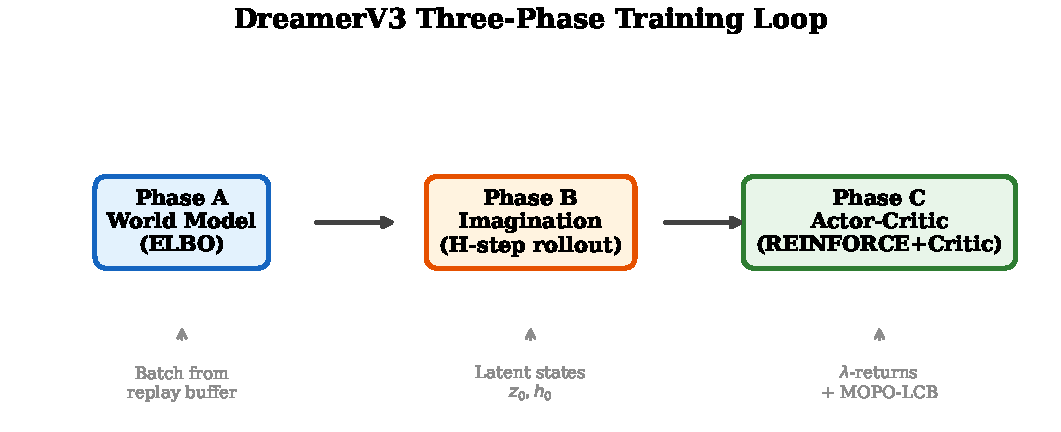
\includegraphics[width=0.9\textwidth]{figures/training_loop.pdf}
\caption{The DreamerV3 three-phase training loop. Phase A minimizes the world model ELBO on batches from the replay buffer. Phase B unrolls the model in latent space using the actor policy. Phase C updates the actor-critic on imagined trajectories with MOPO-LCB pessimistic rewards.}
\label{fig:training-loop}
\end{figure}

The training procedure follows \dreamer{}'s three-phase structure \citep{hafner2023dreamerv3}.

\textbf{Phase A: World model ELBO minimization.} Each step samples $B = 32$ sequences of length $T = 64$ from the replay buffer. The world model loss is
\begin{equation}
\mathcal{L} = \beta_{\text{pred}} \cdot (\mathcal{L}_{\text{recon}} + \mathcal{L}_{\text{reward}} + \mathcal{L}_{\text{continue}}) + \mathcal{L}_{\text{KL}}
\end{equation}
where $\beta_{\text{pred}} = 1.0$. The reconstruction loss is the mean squared error between the decoder output and $\symlog(x_t)$:
\begin{equation}
\mathcal{L}_{\text{recon}} = \frac{1}{2} \| \symlog(x_t) - \hat{x}_t \|^2
\end{equation}
The reward loss is categorical cross-entropy against soft twohot labels encoding $\symlog(r_t)$:
\begin{equation}
\mathcal{L}_{\text{reward}} = -\sum_i \ell_i \log \hat{p}_i
\end{equation}
where $\ell_i$ are the twohot weights and $\hat{p}_i$ are the softmax probabilities.

The continue loss is binary cross-entropy for store closures and product discontinuations:
\begin{equation}
\mathcal{L}_{\text{continue}} = \text{BCE}(\hat{c}_t, 1 - \text{done}_t)
\end{equation}

The KL term uses balanced loss with free bits:
\begin{equation}
\mathcal{L}_{\text{KL}} = \beta_{\text{dyn}} \cdot \max(1, \KL[\sg(q) \| p]) + \beta_{\text{rep}} \cdot \max(1, \KL[q \| \sg(p)])
\end{equation}
with $\beta_{\text{dyn}} = 0.5$, $\beta_{\text{rep}} = 0.1$, and free bits of 1 nat per categorical. The 5:1 asymmetry prevents posterior collapse.

\textbf{Phase B: Imagination rollout.} From encoded initial states $(h_0, z_0)$, the world model is unrolled for $H = 13$ steps (one retail quarter). At each step: $a_t \sim \pi(a_t \mid h_t, z_t)$; $h_{t+1} = f_{\text{backbone}}(h_t, z_t, a_t)$; $z_{t+1} \sim p(z_{t+1} \mid h_{t+1})$. The reward used for the actor is $r_{\text{pessimistic}}$. Lambda-returns are computed backward with $\gamma = 0.95$ and $\lambda = 0.95$:
\begin{equation}
R^\lambda_T = v_\psi(s_T), \quad R^\lambda_t = r_t + \gamma c_t \left( (1-\lambda) v_\psi(s_{t+1}) + \lambda R^\lambda_{t+1} \right)
\end{equation}
Returns are normalized by percentile: $R_{\text{norm}} = R^\lambda / \max(1, P_{95} - P_5)$ with EMA decay 0.99.

\textbf{Phase C: Actor-critic update.} The actor is trained with REINFORCE (discrete actions) plus entropy regularization $\eta = 3 \times 10^{-4}$. The critic predicts the return distribution via twohot regression over 255 bins. An EMA slow critic (decay 0.98) provides regularization. Adam optimizer with learning rates $1 \times 10^{-4}$ (world model), $3 \times 10^{-5}$ (actor and critic), and gradient clipping at 1000 (world model) and 100 (actor and critic).

\begin{algorithm}[t]
\caption{\dreamprice{} Three-Phase Training Loop}
\label{alg:training}
\begin{algorithmic}[1]
\STATE \textbf{Input:} Offline dataset $\mathcal{D}$, replay buffer $R$, replay sampler (70\% uniform quarterly strata, 30\% recent 2 years)
\STATE Initialize world model $\phi$, actor $\theta$, critic $\psi$, slow critic $\psi'$
\FOR{gradient step $= 1, \ldots, N$}
\STATE Sample batch $\{(x_{1:T}, a_{1:T}, r_{1:T})\}$ from $R$
\STATE \textbf{Phase A:} Encode $z_t \sim q_\phi(z_t \mid x_t)$ for all $t$
\STATE \textbf{Phase A:} Run backbone: $h_t = f_\phi(h_{t-1}, z_{t-1}, a_{t-1})$ (parallel)
\STATE \textbf{Phase A:} Compute prior $p_\phi(z_t \mid h_t)$, rewards $\hat{r}_t$, continue $\hat{c}_t$
\STATE \textbf{Phase A:} Update $\phi$ to minimize $\mathcal{L}_{\text{recon}} + \mathcal{L}_{\text{reward}} + \mathcal{L}_{\text{continue}} + \mathcal{L}_{\text{KL}}$
\STATE \textbf{Phase B:} Encode initial $(h_0, z_0)$ from first $T_0$ steps; unroll $H$ steps with $\pi_\theta$
\STATE \textbf{Phase B:} Compute $r_{\text{pessimistic}} = r_{\text{mean}} - \lambda_{\text{LCB}} r_{\text{std}}$ for each step
\STATE \textbf{Phase B:} Compute lambda-returns $R^\lambda$; normalize by percentile
\STATE \textbf{Phase C:} Update $\theta$ via REINFORCE + entropy on $R^\lambda_{\text{norm}}$
\STATE \textbf{Phase C:} Update $\psi$ via twohot CE on return distribution; $\psi' \leftarrow 0.98 \psi' + 0.02 \psi$
\ENDFOR
\STATE \textbf{Output:} Trained world model $\phi$, actor $\theta$
\end{algorithmic}
\end{algorithm}

\subsection{Data Pipeline}

The Dominick's Finer Foods dataset \citep{dominicks1999} spans 400 weeks (September 1989 to May 1997), 93 stores, and approximately 18,000 unique UPCs across 29 product categories. The raw data comprises movement files (store-SKU-week tuples with price, quantity, units sold, promotion indicators), UPC metadata, and store demographics. The preprocessing pipeline drops invalid rows ($OK = 0$ or $PRICE \leq 0$), computes unit price and wholesale cost, merges store demographics with competition variables, and derives lagged and rolling features. The symlog transform is applied to prices and quantities. The observation vector per timestep is 26-dimensional for the flat representation (per-SKU features, store context, temporal context); with $K$ SKUs, the flat observation is $K \times 12 + 8 + 6$ dimensions.

Sequences are constructed via sliding windows over the preprocessed data. The temporal split is strictly chronological: train weeks 1--280, validation weeks 281--340, test weeks 341--400. No shuffling across time is permitted.

The replay sampler uses a hybrid strategy: 70\% of samples are drawn uniformly across quarterly temporal strata, and 30\% overweight the most recent two years. This balances coverage of the full dataset with emphasis on recent dynamics, which may be more relevant for policy evaluation \citep{agarwal2021deep}.
